%!TEX root = main.tex
% a Identify different factors explaining (causing) the variance in the metric,



We recall from our previous work the definition of the metric used to quantify botnet infection (BNI) problem, namely \textit{BNI attempts} which measures the number of attacks executed daily. In figure ~\ref{fig:isp_legend_area}, we show the output of this metric for different Autonomous Systems (AS) ran by ISPs. It is normalized by the address space of each AS, however, in order to explain the variation between AS\/ISP's in this section we identify, analyze and statistically describe the factors behind the variance of the metric defined before.

\subsection{Identifying the underlying factors}
To successfully identify the factors behind the BNI attempts variance first we would like to give an intuition of how does this security issue propagates within a network. A botnet is more likely to try more infection attempts if a it is either active, big or both. The likelihood infection of a potential zombie machine is mainly influenced by the following two factors: how close the potential new member is (w.r.t. euclidean or geodesic~\cite{geodesic} distance) and how secure is the his system.
The former factor type, the distance between a zombie machine and a potential new member of the botnet might be represented by the geographic distance or the logical distance within a network topology, i.e. the type of network in which the zombie machine is connected (Wifi public hot-spot, home network, enterprise network), the Internet penetration in the country or region (High Internet penetration rate may lead to club effect behaviors~\cite{club_effects}).

The latter factor type, the security of the potential zombie machine might depends on different software and hardware variables, i.e. operative system (OS) and application vulnerabilities, software updates (issued patches of known vulnerabilities for a particular version), hardware reliability (backdoor presence), user awareness.

Furthermore, there are other factors that are not specific of this security issue and, therefore, the variance of the metric but related to human behavior, i.e. seasonal behavior of infection attempts, or related to country reality, i.e. pirate software penetration or illegal content downloads rate.

\begin{figure}[h]
     \caption{Infection attempts per day in different AS of the ISPs normalized by address space and multiplied by $10^9$}
     \label{fig:isp_legend_area}
    \centering
    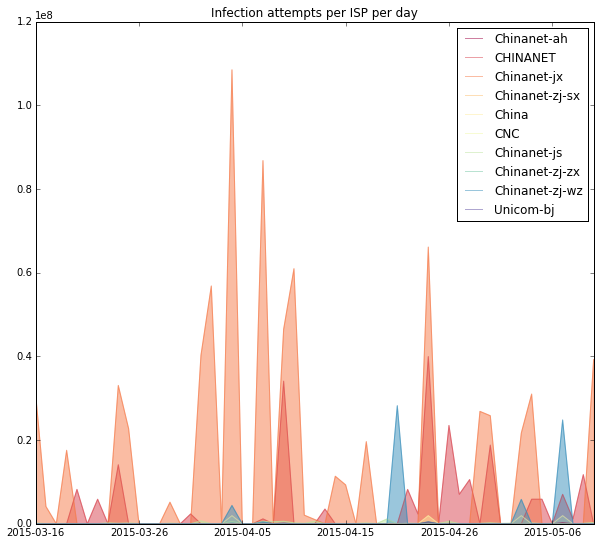
\includegraphics[width=\linewidth]{images/isp_legend_area_norm}
\end{figure}
\begin{figure}[h]
     \caption{Different factors against Botnet infection attempts. In the diagonal the density of the factor is showed.}
     \label{fig:corr2}
    \centering
    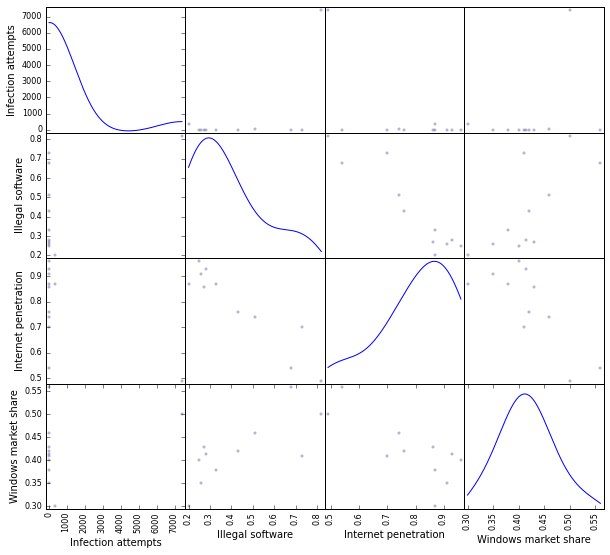
\includegraphics[width=\linewidth]{images/corr_2}
\end{figure}
\subsection{Statistical analysis of the underlying factors}
In figure~\ref{fig:corr2} we show the correlation of different factors such as piracy rate~\cite{pira}, windows OS penetrations,~\cite{win_pen}, Internet penetration~\cite{int_pen}. In table~\ref{tab:corr} we show Pearsons correlation coefficient of the aforementioned variables in relation with the botnet infection attempts.

The motivation to use windows market share as a factor is the high penetration of this OS in the world, i.e., more than 70\% of the OS are Windows distributions~\cite{os_pen}.

In figure~\ref{fig:os_distribution} we show the distribution of OS along different AS, as we might the most common OS in every AS is \textit{Windows 2000}, however, this OS is far to be the most deployed OS~\cite{os_pen} at the end 2014 \textit{Windows 2000} only had less than the 0.05\%.

\begin{table}[]
\centering
\caption{Pearson's correlation}
\label{tab:corr}
\begin{tabular}{l|c}
\multicolumn{1}{c|}{}                          & \textbf{Infection attempts} \\ \hline
\textit{Illegal software} & 0.57                        \\
\textit{Internet penetration}                  & -0.61                       \\
\textit{Windows market share}                  & 0.35                        \\
\textit{Unique IPs}                            & 0.54
\end{tabular}
\end{table}



 We also analyze the relation between the growth in infection per day and the number of unique IPs used. In figure~\ref{fig:corr_1} we can see the strong~\cite{pear_corr} correlation between this two variables and the density of this relation in the diagonal.

We can observe from table~\ref{tab:corr} that the Internet penetration is correlated in a negative way to the number of infection attempts and also to the amount of illegal software in the country. In the other hand, the presence of Windows distribution shows a moderate positive correlation with the infection attempts even when this coefficient was expected to be higher given OS distribution in the dataset. Illegal software presence per country and unique are valuable factor while explaining the behavior of the aforementioned metric since they present a strong correlation with the infection attempts.

The overall behavior of the Botnet Infection attempts are ruled by a variety of factors, we would like to highlight that the country related statistics, i.e. illegal software rate, Internet penetration and Windows market share, present a natural bias originated in the distribution of the dataset used to perform this analysis, however we have the statistical tools and methodology presented before is not data dependent and can produce significant results by explaining the behavior of different datasets representing the same security issue.


\begin{figure}[h]
     \caption{Infection per day vs Unique IPs}
     \label{fig:corr_1}
    \centering
    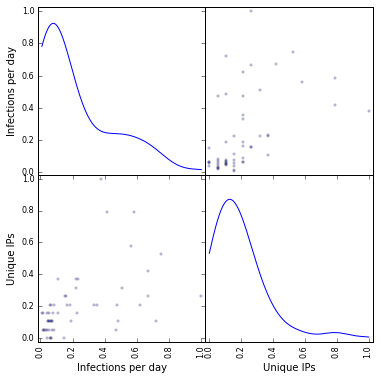
\includegraphics[width=\linewidth]{images/corr_1}
\end{figure}
% \subsubsection{OS}

\begin{figure}[h]
     \caption{OS distribution among the more active ISP's ASs}
     \label{fig:os_distribution}
    \centering
    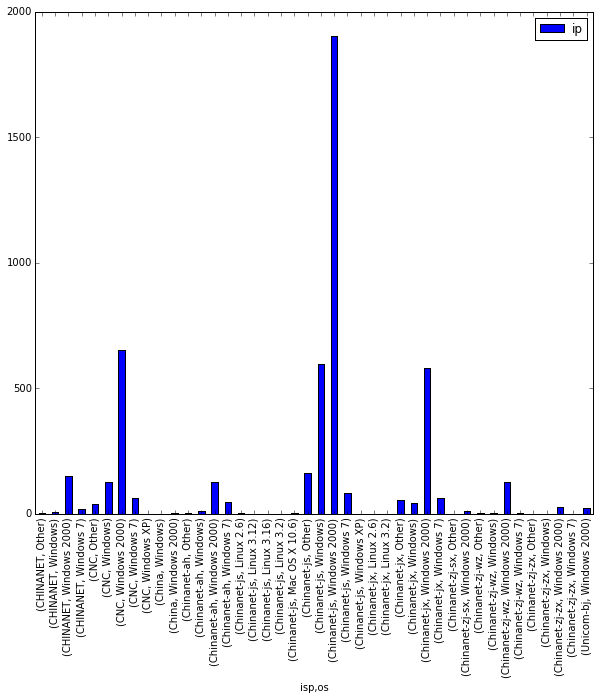
\includegraphics[width=\linewidth]{images/os_isp}
\end{figure}
% section explaining_the_variance_in_botnet_infection_ (end)

